\section{Viewing and Graphics}
\markright{\arabic{section}. Viewing and Graphics}

\subsection{Viewing}
A viewing object manages viewing coordinate system
whose origin is located at the position of a virtual camera,
{\em -z} axis is oriented to the objects observed, and xy-plane is the
projection screen.
Since viewing inherits class cascaded-coords,
it accepts coordinates transformation message
such as {\bf :translate, :rotate} and {\bf :transform}.
Also, it can be attached to another object derived from cascaded-coords,
allowing the simulation of the camera-on-mobile-object system.
The main purpose of viewing is to transform vectors represented in the world
to the camera coordinates system.
The transformation is taken in the opposite direction against usual coordinate
transformation where vectors in the local coordinates are transformed into the
representation in the world.
Therefore, viewing holds the inversed left-handed transformation in
the viewcoords slot, which is usually referred as the viewing coordinate system.

\begin{figure}
\begin{center}
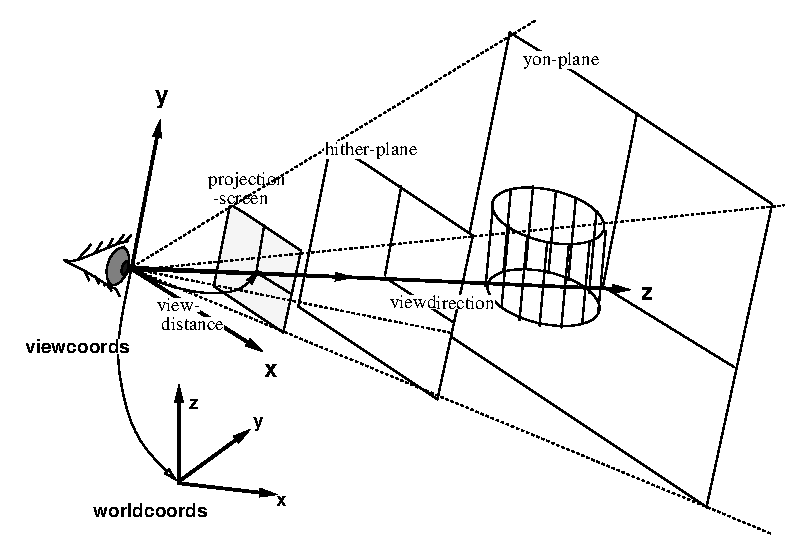
\includegraphics[height=10cm]{fig/viewcoords.ps}
%\epsfile{file=fig/viewcoords.ps,height=10cm}
%\mbox{
%\epsfsize=10cm
%\epsfbox{fig/viewcoords.ps}
%}
\end{center}
\caption{viewing coords and projection planes}
\end{figure}

\begin{refdesc}

\classdesc{viewing}{cascaded-coords}{(viewcoords)}
{defines the viewing transformation.}

\methoddesc{:viewpoint}{}{
returns the position vector of the origin of this viewing.}

\methoddesc{:view-direction}{}{
returns the vector from the origin of the viewing to the center of screen.
This is the z-axis direction of the viewing coordinates.}

\methoddesc{:view-up}{}{
returns y-axis vector of this viewing represented in the world coords.
Y-axis is the upward direction in the viewport.}
\methoddesc{:view-right}{}{
returns x-axis vector of this viewing represented in the world coords.
X-axis is in horizontal direction to the right in the viewport.}

\methoddesc{:look}{from \&optional (to \#f(0 0 0))}{
{\bf :look} conveniently sets the viewing coords as the eye is located
at {\em from} and looking at {\em to} point.}

% \metdesc{:makeviewcoords}{ ax ay az vpoint}
\longdescription{:init}{
\&key  \= :target \hspace{12mm} \=  \#f(0 0 0) \` [method]\\
       \> :view-direction \> nil \\
       \> :view-up \>  \#f(0.0 0.0 1.0)) \\
       \> :view-right \>  nil \\
       \> \&allow-other-keys}{
Since viewing inherits cascaded-coords, all the {\em :init} parameters
such as {\em :pos}, {\em :rot}, {\em :Euler}, {\em :rpy}, etc. can be
used to specify the location and the orientation of the viewing coordinates.
However, viewing's {\em :init} provides easier way to determine the
rotation.
If only {\em :target} is given, view-line (-z axis) is determined to
pass the viewpoint and {\em :target} point, and the {\em :view-right}
vector is determined so that the x-axis is parallel to the xy-plane of the
world coordinates.
You may specify {\em :view-direction} instead of {\em :target} to get the
same effect.
If you give {\em :view-up} or {\em :view-right} parameter in addition to
{\em :target} or {\em :view-direction},
you can determine all the three rotation parameters by yourself.}

\end{refdesc}

\subsection{Projection}

Class {\bf parallel-projection and perspective-projection} process
projection transformation, which is represented with a 4X4 matrix,
i.e., the transformation is taken in the three dimensional homogeneous
coordinates.
Class {\bf projection} is an abstract class for both of these.
Since these projection classes inherit the viewing class,
two coordinates transformation, world-to-viewing and projection
can be performed at the same time.
By sending the {\tt  :project3} message with a 3D vector to a projection object,
a float-vector of four elements is returned.
{\bf Homo2normal} function is used to convert this homogeneous vector
to the normal representation.
The result is a vector represented in so called normalized device coordinates
(NDC), in which a visible vector ranges within -1 to 1
in each of x,y, and z dimensions.
For the simulation of real cameras in a robot world,
the perspective projection is used more often than the parallel-projection.
Perspective-projection defines a few more parameters.
{\tt Screenx} and {\tt screeny} are the sizes of the window on the
viewing plane on which observed objects are projected,
and with the larger screen, the wider space is projected.
{\tt Viewdistance} which defines the distance between the viewpoint
and the viewplane also concerns with the viewing angle.
The larger viewdistance maps the smaller region to the window on the view plane.
{\tt Hither} and {\tt yon} parameters determine the distance to the front and back
depth clipping planes.
Objects outside these two planes are clipped out.
Actually, this clipping procedure is performed by the viewport object.

\begin{refdesc}

\classdesc{projection}{viewing}
{(screenx screeny hither yon projection-matrix)}
{defines projection transformation with a 4x4 matrix.}

\methoddesc{:projection}{\&optional pmat}{
if {\em pmat} is given, it is set to the {\em projection-matrix} slot.
{\bf :projection} returns the current 4x4 projection matrix.}
\methoddesc{:project}{vec}{
{\em Vec} is a three-dimensional homogeneous float-vector of four elements.
{\em Vec} is transformed by projection-matrix,
and the resulted homogeneous representation is returned.}
\methoddesc{:project3}{vec}{
{\em Vec} is a normal 3D float-vector.
{\em Vec} is homogenized and transformed by projection-matrix,
and the resulted homogeneous representation is returned.}
\methoddesc{:view}{ vec}{
applies viewing transformation and projection transformation to {\em vec}
successively.
The resulted homogeneous representation is returned.}
\methoddesc{:screen}{xsize (\&optional (ysize xsize))}{
changes the size of the viewing screen.
The larger the size, the wider view you get.}
\methoddesc{:hither}{ depth-to-front-clip-plane}{
determines the distance from the viewpoint to the front-clipping plane.
Objects before the front-clipping (hither) plane are clipped out.}
\methoddesc{:yon}{ depth-to-back-clip-plane}{
changes the distance between the viewpoint and
the back-clipping plane.
Objects behind the back-clipping (yon) plane are clipped out.}
\methoddesc{:aspect}{\&optional ratio}{
Aspect ratio is the ratio between screen-y and screen-x.
If {\em ratio} is given,
the aspect ratio is changed by setting screen-y to screen-x * {\em ratio}.
{\bf :aspect} returns the current aspect ratio.}
\longdescription{:init}{
\&key \= :hither  \hspace{5mm} \= 100.0 \`[method]\\
      \> :yon    \> 1000.0 \\
      \> :aspect \> 1.0  \\
      \> :screen \> 100.0 \\
      \> :screen-x  \> screen \\
      \> :screen-y \> (* screen-x aspect) \\
      \>  \&allow-other-keys}{
initializes viewing and projection.}

\vspace{5mm}

\classdesc{parallel-viewing}{projection}{()}{
defines parallel projection.
{\bf Hid} (the hidden-line elimination function)
cannot handle parallel projection.}

\metdesc{:make-projection}{}

\classdesc{perspective-viewing}{projection}
{(viewdistance)}{defines a perspective projection transformation.}

\metdesc{:make-projection}{ }
\methoddesc{:ray}{u v}{
returns the normalized direction-vector pointing (u,v) on
the normalized screen from the viewpoint.}
\methoddesc{:viewdistance}{\&optional vd}{
Viewdistance is the distance between viewpoint and the screen.
If {\em vd} is given, it is set to viewdistance.
The viewdistance corresponds to the focal length of a camera.
The greater the viewdistance, the more zoomed-up view you get.
{\bf :viewdistance} returns the current viewdistance.}
\methoddesc{:view-angle}{\&optional ang}{
set screen size so that the prospective angle of the diagonal of the
screen becomes {\em ang} radian.
Note that angles somewhat between 20 degree (approx. 0.4 rad.)
and 50  degree  (0.9 rad.) can generate a natural perspective view.
Wider angle generates a skewed view, and narrower a flat view like
orthogonal (parallel) viewing.
{\bf :view-angle} returns current or new view angle in radian.}
\methoddesc{:zoom}{\&optional scale}{
If {\em scale} is given, the screen is changed relatively to the
current size by {\em scale}
(the viewdistance is unchanged).
If you give 0.5 for {\em scale}, you get two times as wide view as before.
{\bf :zoom} returns new view angle in radian.}
\methoddesc{:lookaround}{alfa beta}{
translates and rotates the viewpoint.
The center of rotation is taken at 
the midst of the hither plane and the yon plane on the viewline.
The viewing coordinates is rotated {\em alfa} radian around world's z-axis
and {\em beta} radian around x-axis locally.
{\bf :lookaround} allows you to move around the object in the center of
viewing.}
\methoddesc{:look-body}{bodies}{
changes view direction, screen sizes, and hither/yon so that all the
{\em bodies} fit in the viewport.
Viewpoint does not change.
View direction is chosen so that the viewing line penetrate the center
of the bounding box of all bodies.}
\metdesc{:init}{ \&key (:viewdistance 100.0) \&allow-other-keys}

\end{refdesc}

\subsection{Viewport}

Class {\bf viewport} performs three-dimensional viewport clipping in
the normalized device coordinates, and maps the result into the device
dependent coordinates.
The viewport is the term representing the visible rectangular area
on a screen.
The physical size (dots in x and y) of a viewport should be given with 
{\bf :init} message as the {\em :width} and {\em :height} arguments.
{\em :xcenter} and {\em :ycenter} arguments determine
the physical location of the viewport.
These two parameters actually decide the location where objects are drawn
on the screen when you are using a primitive display device like tektronics
4014 on which every dimension must be given absolutely to the origin of the
screen.
If you are using more sophisticated display device like Xwindows where
locations can be determined relatively to the parent window, you need not
to change viewport's parameters to move the viewport.
These parameters are independent of the actual display location.

Viewport class assumes the origin of the viewport at the lower-left corner of
the rectangular area and y-axis extends to the upper direction.
Unfortunately, in many window systems and display devices, the origin is taken
at the upper-left corner and y-axis extends to the lower direction.
To work around this problem, a negative value should be given to the
{\em :height} parameter.

\begin{refdesc}

\funcdesc{homo-viewport-clip}{v1 v2}{
{\em V1} and {\em v2}, which are two homogeneous vectors with four elements,
represent a line in 3-D space.
The line is clipped at the boundary of $x=-1, x=1, y=-1, y=1, z=0, z=1$,
and a list of two vectors are returned.
If the line lies completely outside the viewport, NIL is returned.}

\classdesc{viewport}{coordinates}{()}
{viewport transformation maps the NDC (normalized device coordinates)
 to device specific coordinates.
Inheriting the {\bf coordinates} class, the {\tt viewport} defines
the size and the relative position of the projection screen.}

\methoddesc{:xcenter}{\&optional xcenter}{
X coordinates of the center of this viewport.}
\methoddesc{:ycenter}{\&optional ycenter}{
Y coordinates of the center of this viewport.}
\methoddesc{:size}{\&optional size}{
List of sizes in x direction and y direction.}
\methoddesc{:width}{ \&optional width}{width of this viewport.}
\methoddesc{:height}{ \&optional height}{height of this viewport.}
\methoddesc{:screen-point-to-ndc}{p}{
{\em p} is a float-vector representing the location in the physical screen.
{\em p} is transformed into the representation in the normalized-device
coordinates.}
\methoddesc{:ndc-point-to-screen}{p}{
NDC representation in this viewport, {\em p}, is transformed into
the physical address on the screen.}
\methoddesc{:ndc-line-to-screen}{p1 p2 \&optional (do-clip t)}{
Two 3D float-vectors, {\em p1} and {\em p2}, define a line in NDC.
These two end points are transformed to the representation in 
the screen space.
If {\em do-clip} is non-nil, the line is clipped.}
\methoddesc{:init}{\&key (xcenter 100) (ycenter 100) (size 100)
(width 100) (height 100)}
{makes a new viewport object.}

\end{refdesc}

\subsection{Viewer}
To get a drawing  on a screen, four objects are needed:
(1) objects to be drawn, (2) a viewing which defines the viewing coordinates
and the projection, (3) a viewport for clipping in NDC and
the transformation from NDC to physical screen coordinates,
and (4) a viewsurface which performs drawing functions on
a physical display device.
A {\bf viewer} object holds a viewing, a viewport and a viewsurface object,
and controls successive coordinates transformation. 
Functions {\bf draw} and {\bf hid} described in section \ref{Drawings}
use the instances of viewer.

\begin{refdesc}

\classdesc{viewer}{object}
{(eye :type viewint) \\
\> (port :type viewport) \\
\> (surface :type viewsurface)} 
{defines the cascaded coordinates transformation from the viewing via
the viewport to the viewsurface.}

\methoddesc{:viewing}{\&rest msg}{
If {\em msg} is given, {\em msg} is sent to the viewing (eye) object,
Otherwise, the viewing (eye) object is returned.}
\methoddesc{:viewport}{\&rest msg}{
If {\em msg} is given, {\em msg} is sent to the viewport (port) object,
Otherwise, the viewport (port) object is returned.}
\methoddesc{:viewsurface}{\&rest msg}{
If {\em msg} is given, {\em msg} is sent to the viewsurface (surface) object,
Otherwise, the viewsurface (surface) object is returned.}
\methoddesc{:adjust-viewport}{}{
When the size of viewsurface has been changed, {\bf :adjust-viewport}
changes viewport transformation sending a proper message to port.}
\methoddesc{:resize}{width height}{
changes the size of viewsurface by sending :resize message to the viewsurface
and :size message to viewport.}
\methoddesc{:draw-line-ndc}{ p1 p2 \&optional (do-clip t)}{
draws a line whose two end points {\em p1, p2} are defined in NDC.}
\methoddesc{:draw-polyline-ndc}{polylines \&optional color}{
draws polylines whose end points are defined in NDC.}
\methoddesc{:draw-star-ndc}{center \&optional (size 0.01) color}{
draws a cross mark in NDC.}
\methoddesc{:draw-box-ndc}{low-left up-right \&optional color}{
draws a rectangle in NDC.}
\methoddesc{:draw-arc-ndc}{point width height angle1 angle2 [color]}{
draws an arc in NDC.
The viewsurface object bound in this viewer must accept {\bf :arc} message.}
\methoddesc{:draw-fill-arc-ndc}{ point width height angle1 angle2 [color]}{
draws a filled-arc in NDC.}
\methoddesc{:draw-string-ndc}{position string [color]}{
draws {\em string} at {\em position} defined in NDC.}
\metdesc{:draw-image-string-ndc}{position string [color]}
\metdesc{:draw-rectangle-ndc}{position width height [color]}
\metdesc{:draw-fill-rectangle-ndc}{point width height [color]}
\methoddesc{:draw-line}{p1 p2 \&optional (do-clip t)}{
draws a line whose two end points {\em p1, p2} are defined in the world
coordinates.}
\methoddesc{:draw-star}{position \&optional (size 0.01) color}{
draws a cross at {\em position} located in the world.}
\methoddesc{:draw-polyline}{vlist \&optional color}{
draws polylines whose end points {\em vlist} are defined in the world.}
\methoddesc{:draw-box}{center \&optional (size 0.01)}{
draws a rectangular at {\em center}in the world.}
\methoddesc{:draw-arrow}{p1 p2}{
draws an arrow from {\em p1} to {\em p2}.}
\metdesc{:draw-edge}{edge}
\metdesc{:draw-edge-image}{edge-image}
\metdesc{:draw-faces}{face-list \&optional (normal-clip nil)}
\metdesc{:draw-body}{body \&optional (normal-clip nil)}
\methoddesc{:draw-axis}{coordinates \&optional size}{
draws coordinates axes whose length is {\em size}.}
\methoddesc{:draw}{\&rest things}{
draws 3D geometric objects.
If the object is a 3D float-vector, a small cross is drawn at the position.
If it is a list of 3D float-vectors, it is taken as a polyline.
If {\em thing} accepts {\tt :draw} message,
the method is invoked with this viewer as its argument.
If the object defines {\tt :drawners} method,
the {\bf :draw} message is sent to the result of {\tt :drawners}.
{\tt Line, edge, polygon, face}, and {\tt body} objects are drawn
by corresponding {\em :draw-xxx} methods defined in viewer.}
\methoddesc{:erase}{\&rest things}{
draws {\em things} with background color.}
\methoddesc{:init}{\&key :viewing :viewport :viewsurface}{
sets {\em viewing, viewport} and {\em viewsurface} to {\tt eye, port},
and {\tt surface} slots of this viewer.}

\longdescription{view}{\&key \= (size 500) (width size) (height size)
\`[function] \\
\> (x 100) (y 100) \\
\> (title "eusx") \\
\> (border-width 3) \\
\> (background 0) \\
\> (viewpoint \#f(300 200 100)) (target \#f(0 0 0)) \\
\> (viewdistance 5.0)  (hither 100.0) (yon 10000.0) \\
\> (screen 1.0) (screen-x screen) (screen-y screen) \\
\> (xcenter 500) (ycenter 400) \\}
{creates a new viewer and pushes it in *viewers* list.}

\end{refdesc}

\newpage
\subsection{\label{Drawings}Drawings}

\begin{refdesc}

\funcdesc{draw}{[viewer] \&rest thing}{
draws {\em thing}s in {\em viewer}.
{\em Thing} can be any of coordinates, body, face, edge, float-vector,
list of two float-vectors.
If you are running {\tt eusx}, 
{\tt (progn (view) (draw (make-cube 10 20 30)))}
 draws a cube in a xwindow.}

\funcdesc{draw-axis}{[viewer] [size] \&rest thing}{
draws coordinate-axes of {\em thing}s in {\em viewer} with {\em size}
as the length of each coordinates-axis.
{\em Thing} can be any object derived from coordinates.}

\funcdesc{draw-arrow}{p1 p2}{
draws an arrow pointing from p1 to p2 in {\tt *viewer*}.}

\funcdesc{hid}{[viewer] \&rest thing }
{draws hidden-line eliminated image in {\em viewer}.
{\em Thing} can be of face or body.}

\funcdesc{hidd}{[viewer] \&rest thing }{
is same as {\bf hid}, except that {\bf hidd} draws hidden lines
with dashed-lines.}

\funcdesc{hid2}{body-list viewing}{
Generate hidden-line eliminated image represented by edge-image objects.
The result is bound to {\bf *hid*}.}

\funcdesc{render}{\&key bodies faces (viewer *viewer*) (lights *light-sources*)\\
(colormap *render-colormap*) (y 1.0)}{
does ray-tracing for {\em bodies} and {\em faces} and generates
hidden-surface removed images.
viewing, viewport, and viewsurface are taken from {\em viewer}.
{\em lights} is a list of {\tt light-source} objects.
{\em colormap} is xwindow's colormap object.
Each of bodies and faces must have color attribute assigned.
This can be done by sending {\tt :color} message with the name of
color LUT defined in the {\em colormap}.
Currently this function works only in Xlib environment.
See examples in {\tt demo/renderdemo.l}.}

\funcdesc{make-light-source}{pos \&optional (intensity 1.0)}{
make a light-source object located at {\em pos}.
{\em intensity} is magnifying ratio which multiplies default light
intensity. In order to determine the intensity more precisely,
use {\tt :intensity} method of a light-source.}

\macrodesc{tektro}{file \&rest forms}{
opens file for {\tt *tektro-port*} stream, and evaluates forms.
This is used in order to redirect the output of tektro drawings to a file.}

\macrodesc{kdraw}{file \&rest forms}{
{\bf Kdraw} is a macro to produce a [ik]draw-readable postscript file.
{\bf Kdraw} opens {\em file} in {\tt :output} mode,
makes a kdraw-viewsurface and a viewport with which {\tt *viewer*} is replaced,
and evaluates {\em forms}.
Each of {\em forms} is a call to any of drawing functions like {\tt draw} or {\tt hid}.
Drawing messages from these forms are redirected to a {\tt kdraw-viewsurface}, 
which transforms the messages into postscript representations
that {\tt idraw} or {\tt kdraw} can recognize, and stores them in {\em file}.
When  {\tt idraw} or {\tt kdraw} is invoked and {\em file} is opened,
you see the identical figure you drew in a EusViewer window.
The figure can be modified by {\tt idraw}'s facilities,
and the final drawing can be incorporated into a \LaTeX document
using the {\tt epsfile} environment.}

\macrodesc{pictdraw}{file \&rest forms}{
{\bf Pictdraw} is a macro to produce picture files in the Macintosh
PICT format. 
% {\bf Pictdraw} opens {\em file} in {\tt :output} mode,
% \mbox{
% \epsfsize=10cm
% \epsfbox{environment}}
}

\macrodesc{pictdraw}{file \&rest forms}{
{\bf Pictdraw} is a macro to produce picture files for Macintosh
in PICT format. 
{\bf Pictdraw} opens {\em file} in {\tt :output} mode
makes a pictdraw-viewsurface and a viewport with which {\tt *viewer*} is replaced,
and evaluates {\em forms}.
Each of {\em forms} is a call to any of drawing functions like {\tt draw} or {\tt hid}.
Drawing messages from these forms are redirected to a {\tt kdraw-viewsurface}, 
which transforms the messages into PICT format
that {\tt macdraw} or {\tt teachtext} of Macintosh can recognize,
and stores them in {\em file}.
}

\funcdesc{hls2rgb}{hue lightness saturation \&optional (range 255)}{
Color representation in HLS (Hue, Lightness, and Saturation)
is converted to RGB representation.
HLS is often referred to as HSL.
{\em Hue} represents a color around a rainbow circle (from 0 to 360).
0 for red, 45 for yellow, 120 for green, 240 for blue, 270 for magenta, 
and 360 again for red, etc.
{\em Lightness} is a value between 0.0 and 1.0, representing
from black to white.
The color of lightness value of 0 is always black regardless to
the hue and saturation, and the lightness value 1.0 is always white.
{\em Saturation} is a value between 0.0 and 1.0, and represents the
strength of the color. 
The greater the saturation value, the divider the color,
and small saturation values generate weak, dull tone colors.
{\em Range} limits the RGB values.
If you are using a color display which can assign 8bit value to each of
red, green and blue, {\em range} should be 255.
If you use Xwindow, which virtually assigns 16bits integers to RGB,
you should specify {\em range} to 65535.
Note the difference between HSV and HLS.
In HLS, vivid (rainbow) colors are defined with lightness=0.5.}
\funcdesc{rgb2hls}{red green blue \&optional (range 255)}{
RGB representation of a color is converted into the corresponding
representation in HLS.}

\end{refdesc}

\subsection{Animation}
\index{animation}
EusLisp's animation facility provides the pseudo real-time
graphics on stock workstations without graphics accelerators.
The basic idea is the quick playback of a series of images which have been
generated after long computation.
Images are retained in two ways:
one is to keep a number of xwindow pixmaps each of which holds a complete
pixel image, and the other is to keep line segment data obtained by
hidden-line elimination.
The former is faster and the only way for rendered images,
but not suitable for a long animation since it requires much memory
in the X server.
The latter is more memory efficient and suitable for storing data in disks,
but the performance is degraded
when the number of line segments increases.

In either way, the user provide a function which gives new configurations
to the objects to be drawn and generates drawing on {\tt *viewer*}.
{\bf pixmap-animation} calls this function as many times as
specified by the {\em count} argument.
After each call, the content of {\tt *viewsurface*}, which is assumed to
be an xwindow, is copied to a newly created Xwindow pixmap.
These pixmaps are played back by {\bf playback-pixmaps}.
Similarly, {\bf hid-lines-animation} extracts visible line segments
from the result of {\bf hid}, and accumulates them in a list.
The list is then played back by {\bf playback-hid-lines}.

Following functions are defined in {\tt llib/animation.l}, and
{\tt demo/animdemo.l} contains a sample animation program
using {\bf hid-lines-animation} on the ETA3 manipulator model.

\begin{refdesc}
\macrodesc{pixmap-animation}{count \&rest forms}{
{\em forms} are evaluated {\em count} times.
After each evaluation, the content of {\tt *viewsurface*} is copied 
in a new pixmap. A list of {\em count} pixmaps is returned.}
\funcdesc{playback-pixmaps}{pixmaps \&optional (surf *viewsurface*)}{
Each pixmap in the {\em pixmaps} list is copied to {\em surf} successively.
% placing {\em wait} micro seconds interval in-between.
}

\macrodesc{hid-lines-animation}{count \&rest forms}{
{\em forms}, which are assumed to include call(s) to {\bf hid},
are evaluated {\em count} times.
After each evaluation, 
the result of {\bf hid} held in {\bf *hid*} is scanned and visible segments
are collected in a list of point pairs.
A list of length {\em count} is returned.}
\funcdesc{playback-hid-lines}{lines \&optional (view *viewer*)}{
{\em lines} is a list of lists of point pairs.
draws lines successively on {\em view}.
Double buffering technique allocating another pixmap 
is used to generate flicker-free animation.}

\funcdesc{list-visible-segments}{hid-result}{
collects visible segments from the list of edge-images {\em hid-result}.}

\end{refdesc}

\newpage
